\chapitre{Autre}
\sousChapitre{Autre}
\uuid{djCi}
\titre{Classification des points d'un triangle}
\theme{réseaux de neurones}
\auteur{Maxime NGUYEN}
\organisation{AMSCC}
\datecreate{2024-12-13}
\contenu{
	
\texte{ 	On souhaite construire un réseau de neurones qui réalise une classification des points du plan $\R^2$ selon que ces points appartiennent ou non au triangle $T$ dont les sommets sont les points de coordonnées respectives $(-1,-1),(-1,1),(1,1)$ comme ci-dessous.
	
	\begin{center}
		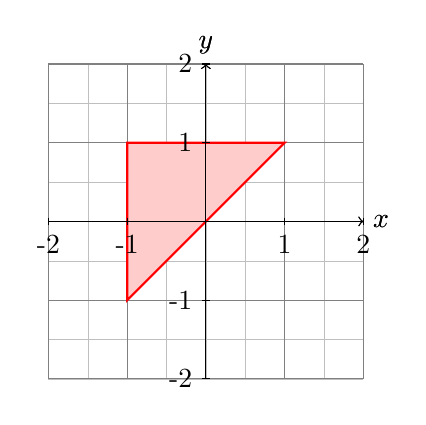
\begin{tikzpicture}[scale=1]
			
			% Grille avec un pas de 0.2 en gris clair
			\draw[step=0.5,lightgray,very thin] (-2,-2) grid (2,2);
			\draw[step=1,gray, thin] (-2,-2) grid (2,2);
			% Axes
			\draw[->] (-2,0) -- (2,0) node[right] {$x$};
			\draw[->] (0,-2) -- (0,2) node[above] {$y$};
			% Dessin du triangle
			\filldraw[thick,red,fill=red!20] (-1,-1) -- (-1,1) -- (1,1) -- cycle;
			% Axes
			\draw[->] (-2,0) -- (2,0) node[right] {$x$};
			\draw[->] (0,-2) -- (0,2) node[above] {$y$};
			
			% Ticks sur l'axe x
			\foreach \x in {-2,-1,1,2} {
				\draw (\x,0.05) -- (\x,-0.05) node[below] {\x};
			}
			% Ticks sur l'axe y
			\foreach \y in {-2,-1,1,2} {
				\draw (0.05,\y) -- (-0.05,\y) node[left] {\y};
			}
			
			
			
			
		\end{tikzpicture}
	\end{center} }
	
	\begin{enumerate}
		\item \question{ Démontrer que le perceptron défini ci-dessous réalise l'opération logique $x$ ET $y$ ET $z$ où $(x,y,z) \in \{0,1\}^3$. 
		
		\begin{center}
			\begin{tikzpicture}[scale=0.3, font=\scriptsize]
				
				\draw[thick,fill=black!10] (0,0) circle (3);
				\draw[ultra thick]  (150:3) -- (150:8)node[pos=0.2,above]{$1$} node[left]{$x$};
				\draw[ultra thick]  (170:3) -- (170:8)node[pos=0.2,above]{$1$} node[left]{$y$};
				\draw[ultra thick]  (190:3) -- (190:8)node[pos=0.2,above]{$1$} node[left]{$z$};
				\draw[-o,ultra thick]  (210:3) -- (210:8) node[pos=0.2,below]{$-3$};
				\draw[->,>=latex,ultra thick] (0:3) --  (8,0);
				\node[below right] at (-15:3) {$H$};
				
			\end{tikzpicture}  
		\end{center} }
	\reponse{
Si $(x,y,z) = (1,1,1)$ alors $x$ ET $y$ ET $z$ vaut $1$, $0$ dans tous les autres cas. 

Or ce perceptron renvoie $1$ si et seulement si $x+y+z \geq 3$. Donc si $x=y=z=1$ alors la sortie vaut $1$. Si $x=0$ ou $y=0$ ou $z=0$ alors $x+y+z \leq 2 < 3$ et la sortie vaut $0$.
}
		\item \question{ En déduire un réseau de neurones prenant un vecteur $(x,y) \in \R^2$ en entrée et renvoyant 
		$1$ si $(x,y) \in T$, $0$ sinon.  }
	\reponse{ 
		Le triangle est l'intersection de trois demi plans définis par ces inéquations : 
		$\begin{cases}
			x + 1 \geq 0 \\
			-y +1 \geq 0 \\
			-x + y \geq 0
		 \end{cases}$
		 d'où le réseau à deux couches suivant où chaque perceptron de la première couche réalise une inéquation et celui de la seconde couche réalise l'intersection :
		 
\begin{tikzpicture}[scale=1.5]
\def\layersep{2cm}
\tikzstyle{every pin edge}=[thick]
\tikzstyle{neuron}=[circle,fill=black!25,minimum size=12pt,inner sep=0pt]
\tikzstyle{entree}=[];
\tikzstyle{input neuron}=[neuron, fill=green!50];
\tikzstyle{output neuron}=[neuron, fill=red!50];
\tikzstyle{hidden neuron}=[neuron, fill=blue!50];
\tikzstyle{annot} = [text width=4em, text centered]

% Entree
\node[entree,blue] (E-1) at (-\layersep,-0.5) {$x$};
\node[entree,blue] (E-2) at (-\layersep,-2.5) {$y$};

% Premiere couche
\node[input neuron] (I-1) at (0,0) {};
\node[input neuron] (I-2) at (0,-1.5) {};
\node[input neuron] (I-3) at (0,-3) {};

\node[below right=0.8ex,scale=0.7] at (I-1) {};
\node[below right=0.8ex,scale=0.7] at (I-2) {};
\node[below right=0.8ex,scale=0.7] at (I-2) {};

% \node[above right=0.8ex,blue] at (I-1) {$s_1$};
% \node[above right=0.8ex,blue] at (I-2) {$s_2$};
% \node[above right=0.8ex,blue] at (I-3) {$s_3$};

%Seconde couche et sortie
\node[output neuron] (O) at (\layersep,-1.5 cm) {};
\node[below right=0.8ex,scale=0.7] at (O) {};

% Arrete et poids
\path[thick] (E-1) edge node[pos=0.8,above,scale=0.7]{$1$} (I-1) ;
\path[thick] (E-2) edge node[pos=0.8,above left,scale=0.7]{$0$} (I-1);
\draw[-o,thick] (I-1) to node[midway,below right,scale=0.7]{$1$} ++ (-110:0.8);

\path[thick] (E-1) edge node[pos=0.8,above,scale=0.7]{$0$} (I-2);
\path[thick] (E-2) edge node[pos=0.8,above,scale=0.7]{$-1$} (I-2);
\draw[-o,thick] (I-2) to node[midway,below right,scale=0.7]{$1$} ++ (-130:0.8);

\path[thick] (E-1) edge node[pos=0.9,above right,scale=0.7]{$-1$} (I-3);
\path[thick] (E-2) edge node[pos=0.8,above,scale=0.7]{$1$} (I-3);
%\draw[-o,thick] (I-3) to node[midway,below right,scale=0.7]{$3$} ++ (-130:0.8);

\path[thick] (I-1) edge node[pos=0.8,above,scale=0.7]{$1$} (O);
\path[thick] (I-2) edge node[pos=0.8,below,scale=0.7]{$1$}(O);
\path[thick] (I-3) edge node[pos=0.8,below,scale=0.7]{$1$}(O);
\draw[-o,thick] (O) to node[midway,below right,scale=0.7]{$-3$} ++ (-110:0.8) ;

% Sortie
\draw[->,thick] (O)-- ++(1,0) node[right,blue]{$F(x,y)$};

\end{tikzpicture}  	

Toutes les fonctions d'activation sont la fonction Heaviside.
 }
		\item \question{ Soit $P$ un polygône convexe du plan à 10 côtés. Décrire l'architecture d'un réseau de neurones permettant de réaliser une classification des points appartenant à l'intérieur de ce polygône.  }
		\reponse{ 
	Un polygône convexe est l'intersection de $10$ demi plans. Pour le réaliser, on peut décrire un réseau de neurones à deux couches prenant en entrée un vecteur $(x,y) \in \R^2$ : 
	\begin{itemize}
		\item La première couche est constituée de $10$ neurones réalisant les $10$ demi plans ;
		\item La seconde couche est constituée de $1$ neurone réalisant la fonction logique \texttt{ET} sur $\{0,1\}^{10}$ : il suffit de prendre par exemple : 
		
				\begin{center}
			\begin{tikzpicture}[scale=0.3, font=\scriptsize]
			
			\draw[thick,fill=black!10] (0,0) circle (3);
			\draw[ultra thick]  (150:3) -- (150:8)node[pos=0.2,above]{$1$} node[left]{$x_1$};
			\draw[ultra thick]  (170:3) -- (170:8)node[pos=0.2,above]{$...$} node[left]{$...$};
			\draw[ultra thick]  (190:3) -- (190:8)node[pos=0.2,above]{$1$} node[left]{$x_{10}$};
			\draw[-o,ultra thick]  (210:3) -- (210:8) node[pos=0.2,below]{$-10$};
			\draw[->,>=latex,ultra thick] (0:3) --  (8,0);
			\node[below right] at (-15:3) {$H$};
			
			\end{tikzpicture}  
		\end{center}
	avec $(x_1,\cdots,x_{10}) \in \{0,1\}^{10}$ en entrée, les poids $(a_1,\cdots,a_{10}) = (1,\cdots,1)$, un biais $a_{11} = -10$ et une fonction d'activation Heaviside.
	\end{itemize}	
	 }
	\end{enumerate}
	
}
